\subsection{Interfaz del Dashboard}
Al iniciar sesión, la primera página que ve el cliente es el dashboard. En este dashboard se muestra un mensaje personalizado para el cliente y las campañas activas de Mezfer (Ver Figura 7).

    \begin{figure}[H]
        \begin{center}
            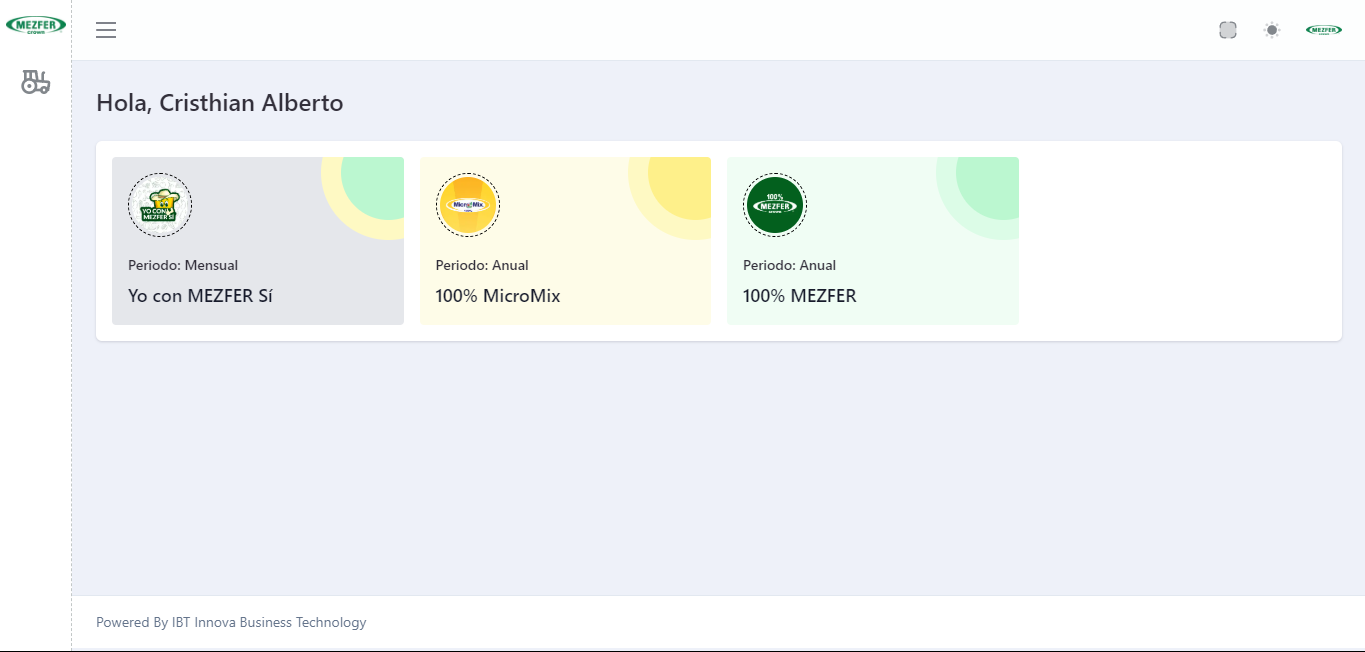
\includegraphics[scale=0.35]{img/actividades/dashboard-cliente/dashboard-cliente.png}
            \caption{Dashboard de clientes.}
            \label{fig:dashboard-clientes}
        \end{center}
    \end{figure}

Antes de cargar las campañas y el mensaje personalizado, se renderiza un componente llamado ``Skeleton'' que muestra la estructura de la página pero sin ningún contenido, sólo elementos grises que representan que la información se esta cargando. Este componente se muestra en lo que se obtiene la información de la API.

Una vez se haya cargado la información, el Skeleton deja de renderizarse y ahora muestra el mensaje personalizado y las campañas activas en componentes llamados ``Cards''. El cliente puede dar clic a cada una de estas Cards, lo que lo llevará a otra página donde se muestran todos los detalles de la campaña, pero esto se explicará más adelante.